
\centerline{\textbf{ \LARGE Other CSO Topics}}

\begin{enumerate}

    \item Instruction Format
    \begin{enumerate}
      \item Opode(n-bits) = { \large \(  \mathbf{ 2^n }\) } types of instructions(operations)
      \item Immediate Operand(t-bits), Register(k-bits), Memory Address(m-bits)

          \begin{myTableStyle} \begin{tabular}{ |m{14cm}| } \hline
             \begin{center} 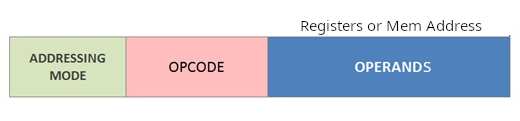
\includegraphics[scale=1]{./images/Instruction-Format.jpg} \end{center}\\ \hline
          \end{tabular} \end{myTableStyle} \vspace{0.08in}
    \end{enumerate}
    \item A processor has 40 distinct instructions and 24 general purpose registers.
             A 32-bit instruction word has an opcode, two register operands and an immediate operand.
             \\ (a) 5-bits to index 24 register
             \\ (b) 6-bis to index 40 opcode
             \\ (c) Instruction(32 bit) = opcode(6) + R1(5) + R2(5) + Immediate Operand(16)

    \item Microprocessor - 8085.
    \begin{enumerate}
        \item \( \overline{INTA} \)  is interupt acknowledgement signal. Whenever the microprocessor
              receives interrupt signal. It has to be acknowledged. This acknowledgement is done by
              \( \overline{INTA} \).  Processor saves the address of next instruction into the STACK
              and an interrupt service subroutine begins. CALL instruction saves procedure linking
              information on the stack and branches to the procedure (called procedure) specified
              with the destination (target) operand.

        \item INTR is an interrupt request signal it's full form is Interrupt Request.

        \item READY signal indicates that the device is ready to send or receive data.
              If READY is low, then the CPU has to wait for READY to go high.

        \item HOLD signal indicates that another master is requesting the use of the address and data buses.

        \item HLDA (HOLD Acknowledge) - It indicates that the CPU has received the HOLD request and it will
              relinquish the bus in the next clock cycle. HLDA is set to low after the HOLD signal is removed.

    \end{enumerate}

    \item CISC Vs RISC

    \item Control Unit design :
    \begin{enumerate}
      \item Types : Hard wired, Micro-programmed(horizontal, vertical).
      \item Hard wired control involves only hardware and it is the fastest.
      \item In horizontal microprogramming control signals are not encoded.
      \item In vertical microprogramming signals are encoded to save memory. So, it is slower because
            decoding of signals is not required.
      \item Micro-programmed CU needs control memory to store micro-instructions.
    \end{enumerate}

    \item Horizontal microprogramming.
      \begin{enumerate}
      \item does not require use of signal decoders
      \item results in larger sized microinstructions than vertical microprogramming
      \item uses one bit for each control signal
      \end{enumerate}

    \item Control Memory.
    \begin{enumerate}
      \item Control memory stores \( \mathbf { 2^{10} } \) words.
      \item Each word contains one micro-instruction(MI).
      \item MI(26) = micro-operation(13) + Next\_MI\_Addr(10) + Mux\_Select(3).
      \item MUX select field(Y=3) selects one of the 8 status bits of the MUX.

          \begin{myTableStyle} \begin{tabular}{ |m{14cm}| } \hline
             \begin{center} 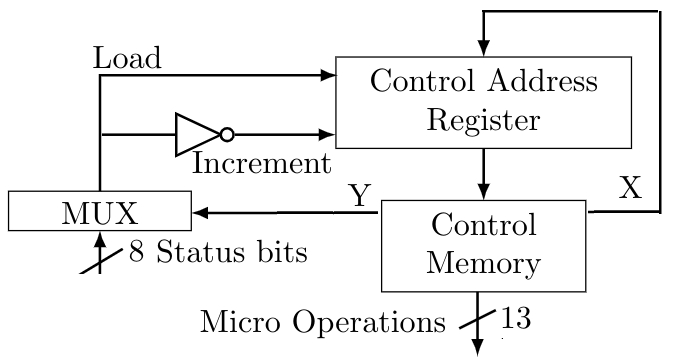
\includegraphics[scale=0.4]{./images/control_memory.jpeg} \end{center}\\ \hline
          \end{tabular} \end{myTableStyle} \vspace{0.08in}
    \end{enumerate}

    \item Data Paths.
    \begin{enumerate}
      \item ALU and Control Unit
          \begin{myTableStyle} \begin{tabular}{ |m{14cm}| } \hline
             \begin{center} 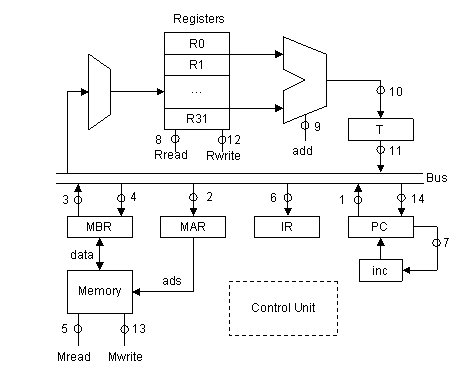
\includegraphics[scale=0.7]{./images/data_paths_02.jpeg} \end{center}\\ \hline
          \end{tabular} \end{myTableStyle} \vspace{0.08in}
    \end{enumerate}

\end{enumerate}
